\chapter{Eksperimen}
Bab ini memaparkan secara kronologis tentang proses eksperimen yang telah dilakukan oleh penulis.

\section{Mengintegrasikan ABS dengan JAVA}
Berdasarkan hasil studi literatur yang telah dilakukan, penulis mengetahui bahwa salah satu fitur yang dimiliki oleh ABS adalah kemampuannya untuk dapat di\textit{compile} kedalam bahasa JAVA sehingga nantinya kode ABS tersebut dapat dijalankan di dalam JAVA Runtime Environment (JRE). Berdasarkan informasi tersebut, penulis menarik kesimpulan bahwa jika penulis membuat sebuah JAVA class yang dibuat secara \textit{native}, maka JAVA Class tersebut akan dapat memanggil class ABS yang sudah di\textit{compile} menjadi JAVA Class juga.\\

Sebelum penulis mencoba untuk mengintegrasikan secara langsung ABS dengan JAVA, penulis mencoba untuk mengetahui hasil kompilasi kode ABS yang diubah kedalam JAVA. berikut adalah kode ABS sederhana yang penulis buat beserta hasil kompilasinya ke dalam kode JAVA.

\begin{lstlisting}[
caption=Kode ABS beserta Main Blocknya,
label={lst:absSederhana},
escapeinside={@}{@}
]
module UserModule;

interface User
{
	String getUsername();
}

class UserImpl implements User
{
	String getUsername() @\label{lst:absString}@
	{
		return "salman"; @\label{lst:absString2}@
	}
}

//ABS Main block
{
	User myUser = new local UserImpl(); @\label{lst:absCreateObject}@
	String username = myUser.getUsername();
}
\end{lstlisting}

\begin{lstlisting}[ 
firstnumber=64,
caption=Hasil kompilasi ABS ke JAVA untuk method getUsername(),
label={lst:absjavaGetUsername},
escapeinside={@}{@},
]
// User.abs:10:2: 
public final abs.backend.java.lib.types.ABSString getUsername() {
    ...
    return abs.backend.java.lib.types.ABSString.fromString("salman"); @\label{lst:absjavaString}@
}
\end{lstlisting}

\begin{lstlisting}[
caption=Hasil kompilasi ABS ke JAVA untuk Main Block,
label={lst:absjavaMainBlock},
escapeinside={@}{@}
]
package UserModule;
public class Main extends abs.backend.java.lib.runtime.ABSObject {
    public static void main(java.lang.String[] args) throws Exception {
        abs.backend.java.lib.runtime.StartUp.startup(args,Main.class);
    }
    public java.lang.String getClassName() { return "Main"; }
    public java.util.List<java.lang.String> getFieldNames() { return java.util.Collections.EMPTY_LIST; }
    public Main(abs.backend.java.lib.runtime.COG cog) { super(cog); }
    public abs.backend.java.lib.types.ABSUnit run() {
         {
            ...
            UserModule.User_i myUser = UserModule.UserImpl_c.__ABS_createNewObject(this); @\label{lst:absjavaCreateObject}@
            
            ...
            abs.backend.java.lib.types.ABSString username = abs.backend.java.lib.runtime.ABSRuntime.checkForNull(myUser).getUsername();
            if (__ABS_getRuntime().debuggingEnabled()) __ABS_getRuntime().getCurrentTask().setLocalVariable("username",username);
        }
        
        return abs.backend.java.lib.types.ABSUnit.UNIT;
    }
}
\end{lstlisting}

Seperti yang terlihat pada kode \ref{lst:absjavaMainBlock} baris \ref{lst:absjavaCreateObject}, terdapat perbedaan pada kode JAVA hasil kompilasi dari ABS dalam membuat \textit{instance} dari sebuah objek. Dalam bahasa JAVA yang standar, untuk dapat membuat \textit{instance} dari sebuah class adalah dengan menggunakan kata kunci \texttt{new} seperti misalnya \texttt{new UserImpl()}. Sedangkan pada kode JAVA hasil kompilasi ABS menggunakan kata kunci \texttt{\_\_ABS\_createNewObject(this)} yang diakses secara \textit{static}.\\

Berdasarkan hasil percobaan tersebut penulis mengetahui bahwa sintaks ABS yang terdapat pada kode \ref{lst:absSederhana} baris \ref{lst:absCreateObject} adalah \textit{equivalent} dengan sintaks JAVA yang terdapat pada kode \ref{lst:absjavaMainBlock} baris \ref{lst:absjavaCreateObject}. Dengan demikian, penulis dapat menyimpulkan bahwa ketika penulis ingin mencoba untuk memanggil class JAVA hasil kompilasi ABS dari class JAVA yang \textit{native} maka penulis harus melakukan pemanggilan fungsi seperti yang terlihat pada kode kode \ref{lst:absjavaMainBlock} baris \ref{lst:absjavaCreateObject} tersebut.\\

Selain terdapat perbedaan dalam cara membuat \textit{instance} dari sebuah class, terdapat pula perbedaan pada tipe data yang digunakan oleh JAVA hasil kompilasi dari ABS dengan JAVA yang \textit{native}. Jika kita melihat kode \ref{lst:absSederhana} baris \ref{lst:absString} dan \ref{lst:absString2} penulis menggunakan sebuah tipe data \texttt{String} seperti layaknya tipe data \texttt{String} pada JAVA. Akan tetapi ketika kode ABS tersebut di\textit{compile} kedalam bahasa JAVA, ternyata tipe data \texttt{String} tersebut diubah menjadi \texttt{ABSString} seperti yang terlihat pada kode \ref{lst:absjavaGetUsername} baris \ref{lst:absjavaString}. Berdasarkan hasil percobaan tersebut penulis berkesimpulan bahwa ketika penulis ingin mengintegrasikan ABS dengan JAVA, penulis perlu melakukan konversi tipe data dari tipe data milik JAVA ABS menjadi tipe data standar JAVA.\\

Kesimpulan yang penulis dapatkan setelah melakukan percobaan ini adalah: (1) bahwa untuk dapat membuat sebuah \textit{instance} dari class JAVA hasil kompilasi ABS tidak dapat dilakukan dengan menggunakan kata kunci \texttt{new} seperti pada JAVA yang \textit{native} dan (2) terdapat perbedaan tipe data antara \textit{native} JAVA dengan JAVA hasil kompilasi ABS sehingga perlu adanya penyesuaian lebih lanjut agar penulis dapat mengintegrasikan ABS dengan \textit{native} JAVA.

\section{Membuat halaman web sederhana menggunakan ABS}
Setelah penulis melakukan percobaan sederhana untuk mengetahui cara mengintegrasikan ABS dengan JAVA, selanjutnya penulis melakukan percobaan untuk dapat membuat halaman web sederhana dengan menggunakan ABS. Seperti yang telah kita ketahui bersama, untuk dapat menampilkan sebuah halaman web pada web browser, dibutuhkan adanya sebuah web server yang nantinya akan dapat melayani permintaan dari web browser. Dalam percobaan ini penulis membuat sebuah web server sederhana dengan menggunakan \texttt{ServerSocket} pada JAVA untuk membuka \textit{port} dan menerima \textit{request} dari \textit{web browser} yang nantinya akan memanggil class JAVA hasil kompilasi ABS untuk mendapatkan halaman web yang diinginkan (lihat gambar \ref{fig:howAbsGenerateHTML}).

\begin{figure}
    \centering
    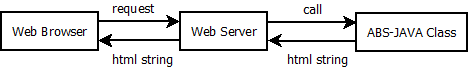
\includegraphics[
        width=0.8\textwidth
    ]{img/request-webserver-abs.png}
    \caption{Bagaimana web server menghasilkan sebuah halaman web}
    \label{fig:howAbsGenerateHTML}
\end{figure}

Untuk dapat mensimulasikan proses seperti yang telah digambarkan pada gambar \ref{fig:howAbsGenerateHTML} di atas, pertama-tama penulis membuat sebuah ABS Module yang fungsinya adalah untuk dapat menghasilkan sebuah halaman sederhana dan memberikannya kepada \textit{web server}. berikut adalah kode ABS yang penulis buat untuk menghasilkan sebuah halaman web:

\begin{lstlisting}[
caption=Kode ABS untuk menghasilkan halaman HTML,
label={lst:absWelcomeView},
]
module ABS.MVC.View.WelcomeView;

interface WelcomeView
{
	String generateView();
}

class WelcomeViewImpl implements WelcomeView
{
	
	String generateView() {		
		String html = "<!DOCTYPE HTML>";
		html = html + "<html>";
		html = html + "<body>";
		html = html + "<h1>Welcome!!</h1>";
		html = html + "Please login <a href='/login.abs'>here</a>";
		html = html + "<br />";
		html = html + "<p>This page was generated from ABS Class</p>";
		html = html + "</body>";
		html = html + "</html>";
		
		return html;
	}
}
\end{lstlisting}

Seperti yang terlihat pada kode \ref{lst:absWelcomeView} di atas, penulis menggunakan \texttt{String} berisikan kode HTML yang disambung-sambung (\textit{concatted String}) untuk menghasilkan sebuah halaman web. Rencananya adalah string yang sudah dihasilkan oleh halaman ABS Module ini nantinya akan diberikan ke \textit{web server} untuk kemudian diberikan ke \textit{web browser} dan ditampilkan ke \textit{user}. Sebagai awalan, penulis membuat sebuah class JAVA yang ditujukan untuk memanggil class JAVA hasil kompilasi ABS tersbeut untuk kemudian ditampilkan di \textit{console} dengan menggunakan \texttt{System.out.println()}. Berikut adalah kode JAVA yang dibuat oleh penulis beserta hasil pemanggilan class ABS-nya.

\begin{lstlisting}[
caption=Kode JAVA untuk memanggil ABS,
label={lst:javaCallABS},
escapeinside={@}{@}
]
package com.fmse.absserver;

public class ABSMain extends ABSObject 
{
    ...
       
    public ABSUnit run() {
        System.out.println("ABSMain running..");
        WelcomeView_i view = WelcomeViewImpl_c.__ABS_createNewObject(this); @\label{lst:javaCreateABSObject}@
        ABSString html = ABSRuntime.checkForNull(view).generateView(); @\label{lst:javaCallABSMethod}@
        System.out.println(html.getString());
        return ABSUnit.UNIT; 
    }
    
    public static void main(String[] args) throws Exception {
        StartUp.startup(new String[0], ABSMain.class);
    }
}
\end{lstlisting}

\begin{figure}
    \centering
    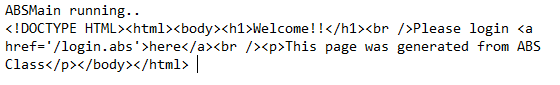
\includegraphics[
        width=0.8\textwidth
    ]{img/java-call-abs-result.png}
    \caption{Hasil dari pemanggilan ABS yang berisikan HTML String}
    \label{fig:javaABSCallResult}
\end{figure}

Terlihat pada kode \ref{lst:javaCallABS} baris \ref{lst:javaCreateABSObject} dan \ref{lst:javaCallABSMethod} di atas, penulis membuat sebuah \textit{instance} dari class \texttt{WelcomView} serta melakukan pemanggilan fungsi \texttt{generateView()} untuk mendapatkan \texttt{String} HTML yang telah dibuat. Hasil dari pemanggilan fungsi \texttt{generateView()} pada class \texttt{WelcomeView} tersebut adalah sebuah \texttt{String} panjang berisikan kode HTML seperti yang terlihat pada gambar \ref{fig:javaABSCallResult}.\\

Setelah penulis berhasil memanggil class JAVA hasil kompilasi ABS untuk mendapatkan HTML String, langkah selanjutnya adalah memberikan HTML String tersebut kepada web browser. Untuk dapat melakukan hal tersebut, penulis akan membuat sebuah web server sederhana dengan menggunakan class \texttt{ServerSocket} pada JAVA. Berikut adalah kode JAVA yang penulis buat untuk dapat menerima request dari \textit{web browser} dan memberikan halaman web yang diinginkan kepada \textit{web browser}.

\begin{lstlisting}[
caption=Potongan kode web server yang memanggil class ABS,
label={lst:javaSimpleWebServer},
escapeinside={@}{@}
]
public class ABSHttpServer extends ABSObject {

    ...
    
    public ABSUnit run() {
        try {
            ServerSocket serverSocket = new ServerSocket(8080); @\label{lst:javaCreateSocket}@
            while(true) {
                Socket remote = serverSocket.accept(); @\label{lst:javaCreateSocket2}@
                BufferedReader in = new BufferedReader(
                        new InputStreamReader(remote.getInputStream()));
                String request = in.readLine();
                String[] protocols = request.split(" ");
                
                ...
                
                if(protocols[1].equals("/")) { @\label{lst:serverStartCallABS}@
                	WelcomeView_i view = WelcomeViewImpl_c.__ABS_createNewObject(this); 
                    html = ABSRuntime.checkForNull(view).generateView().getString();
                    out.println(html);
                } @\label{lst:serverEndCallABS}@
                
                out.flush();
                remote.close();
            }
        }
        catch(Exception e) {
            e.printStackTrace();
        }
        
        return ABSUnit.UNIT;
    }
    
    ...
}
\end{lstlisting}

Pada kode \ref{lst:javaSimpleWebServer} baris \ref{lst:javaCreateSocket} dan \ref{lst:javaCreateSocket2} di atas, terlihat bahwa penulis melakukan pembuatan \texttt{ServerSocket} dan membuka \textit{port} 8080 untuk menerima \textit{request} dari \textit{web browser}. Setelah \textit{web server} menerima \textit{request} dari \textit{web browser}, berikutnya \textit{web server} akan mencocokan URL yang diberikan oleh \textit{web browser} seperti yang terlihat pada gambar \ref{fig:webBrowserRequest}. Apabila URL yang diminta cocok dengan salah satu kondisi yang ada di \textit{web server}, berikutnya \textit{web server} akan melakukan pemanggilan class ABS seperti yang terlihat pada kode \ref{lst:javaSimpleWebServer} baris \ref{lst:serverStartCallABS} - \ref{lst:serverEndCallABS}. Setelah HTML String berhasil diterima oleh \textit{web server} berikutnya akan diberikan ke \textit{web browser} melalui \texttt{OutputStream} pada \texttt{ServerSocket} untuk kemudian ditampilkan di \textit{web browser} seperti yang terlihat pada gambar di bawah ini.

\begin{figure}
    \centering
    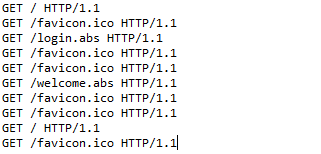
\includegraphics[
        width=0.6\textwidth
    ]{img/web-browser-request.png}
    \caption{Contoh \textit{request} dari \textit{web browser}}
    \label{fig:webBrowserRequest}
\end{figure}

\begin{figure}
    \centering
    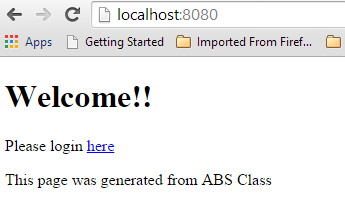
\includegraphics[
        width=0.6\textwidth
    ]{img/abs-welcome-view.png}
    \caption{Halaman web yang dibuat menggunakan ABS}
    \label{fig:javaABSCallResult}
\end{figure}

Sampai pada tahap ini penulis telah berhasil membuat sebuah halaman web sederhana dengan menggunakan ABS. Langkah berikutnya yang penulis lakukan adalah mencoba untuk memetakan ABS kedalam komponen-komponen MVC untuk membuat sebuah MVC Framework.

\section{Memetakan ABS kedalam komponen MVC}
Bagian ini menjelaskan tentang proses pemetaan ABS kedalam komponen Model, View dan Controller. Pada bagian ini juga akan dijelaskan tentang keputusan penulis dalam memilih thymeleaf templating engine sebagai pengganti ABS dalam membuat komponen View pada framework ABS MVC.

\section{Membuat Ant Script untuk mempermudah proses Compile dan Deployment}
Bagian ini menjelaskan tentang proses pembuatan ant script untuk mempermudah proses compile dan deployment dari yang sebelumnya menggunakan menu di eclipse menjadi ke terminal console.

\section{Menerima input POST dan GET dari web browser}
Bagian ini menjelaskan tentang eksperimen yang dilakukan oleh penulis dalam mencari tahu metode seperti apa yang dapat digunakan dalam menerima input HTTP POST dan GET dari web browser.

\section{Membuat Routing configuration}
Bagian ini menjelaskan tentang proses pembuatan routing configuration untuk memetakan setiap url kedalam class controller dan methodnya.